% Q17: 按固定候选 PDF 第1页（印刷页280）重绘；保持原图标注与虚实关系，非比例图。
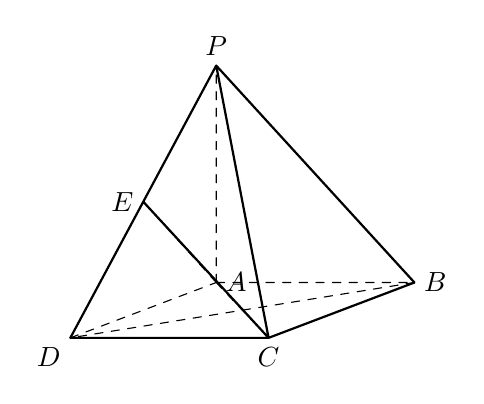
\begin{tikzpicture}[line cap=round,line join=round,scale=0.95]
  \coordinate (A) at (0,0);
  \coordinate (B) at (2.65,0);
  \coordinate (C) at (0.70,-0.74);
  \coordinate (D) at (-1.95,-0.74);
  \coordinate (P) at (0,2.90);
  \coordinate (E) at (-0.975,1.08);

  % 隐藏的底面边、底面对角线、PA 及题图辅助线
  \draw[dashed] (A)--(B) (B)--(D) (D)--(A) (A)--(C) (A)--(P) (A)--(E);
  % 可见棱与题图中的线段 EC
  \draw[thick] (B)--(C) (C)--(D) (P)--(B) (P)--(C) (P)--(D) (E)--(C);

  \node[above] at (P) {$P$};
  \node[right] at (A) {$A$};
  \node[right] at (B) {$B$};
  \node[below] at (C) {$C$};
  \node[below left] at (D) {$D$};
  \node[left] at (E) {$E$};
\end{tikzpicture}
